% !TEX encoding = UTF-8
% !TEX TS-program = pdflatex
% !TEX root = ../tesi.tex

%**************************************************************
\chapter{\textit{License Manager 1.0}}
\label{cap:license-manager}
%**************************************************************

\textit{License Manager 1.0} nasce con lo scopo di creare nuove licenze, eliminando \textit{GenPK} e le problematiche ad esso correlato. Nel corso dello stage, con il delinearsi di nuovi obiettivi, il programma è stato ampliato per poter gestire la maggior parte degli aspetti di una licenza, incluso il monitoraggio. Le funzionalità del Software sono svolte tramite chiamate a Web Service, i quali utilizzano il Database \texttt{DBLicenze} per il salvataggio dei dati.
\\
Inizialmente pensato per un uso interno all'azienda, grazie alle molteplici funzionalità che esso offriva, è stato deciso di distribuire il Software anche ai rivenditori, concedendo loro una maggior capacità operativa.
I rivenditori, per la sicurezza dell'azienda, possono usufruire di operazioni limitate, e le modifiche più rilevanti sono comunicate a \textit{VISIONEIMPRESA} tramite mail.


%**************************************************************
\section{Scopo del prodotto}

Con \textit{License Manager 1.0} si vuole racchiudere in un unico programma la possibilità di gestire completamente le licenze del \textit{Software Gestionale Vision}, dalla creazione all'eliminazione, con la possibilità di effettuare modifiche, ricevere statistiche e monitorare lo stato delle licenze per notare possibili anomalie. 

%**************************************************************

\section{Tipologie di utenti}

\textit{License Manager 1.0} gestisce due tipologie di utente, \textit{Admin} e \textit{Guest}.

\begin{itemize}
\item \textbf{\textit{Admin}}: ha a disposizione tutte le funzionalità senza limitazioni, ed è ideato per i soli membri dell’azienda. Un utente di questo tipo può visualizzare e modificare tutte le licenze, indipendentemente da chi le abbia create;

\item \textbf{\textit{Guest}}: ha a disposizione tutte le funzionalità ma con alcune limitazioni. Questo tipo di utente è creato per ogni rivenditore, in modo che esso possa gestire solo le licenze da esso vendute, senza interferire con le licenze create dall’azienda o da altri rivenditori. Ad ogni \textit{Guest} è associato un \texttt{Codice Utente}, ossia un codice definito per lo specifico rivenditore, e più \textit{Guest} possono avere lo stesso \texttt{Codice Utente}, poiché un rivenditore potrebbe voler affidare la gestione delle proprie licenze ad utenti diversi.
\end{itemize}


%**************************************************************
\section{Autenticazione}
Poiché il programma si propone di gestire diverse tipologie di utenti è stato implementato un sistema di autenticazione. In Figura \ref{auth} è mostrato il form di autenticazione, visibile all'avvio del programma.

\begin{figure}[!h] 
    \centering 
    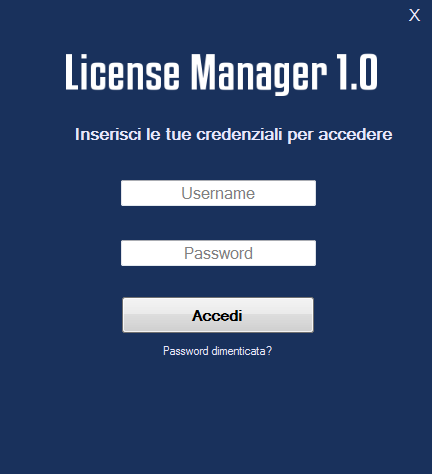
\includegraphics[width=0.5\columnwidth]{LicenseManager/auth} 
    \caption{License Manager 1.0 - Form di autenticazione}
    \label{auth}
\end{figure}

L’utente, per accedere, deve inserire il proprio \texttt{Username} e la \texttt{Password}, e cliccare su "Accedi".\\
Solo gli \textit{Admin} possono creare gli utenti, scegliendone l’username, un indirizzo email da associare, e nel caso l’utente sia destinato a un rivenditore è data la possibilità di sceglierne il \texttt{Codice Utente} (o codice rivenditore).
Un utente che ha dimenticato la password è costretto a contattare un \textit{Admin} per chiederne il reset. Se l’\textit{Admin} concede il reset della password, inserendo l’\texttt{Username} e cliccando su "Password dimenticata?" è possibile impostare una nuova Password.\\
Per maggiori dettagli sulla gestione degli utenti si rimanda alla sezione X.X9 “Amministra utenti”.
\newpage


%**************************************************************
\section{Struttura generale del Software}
Dopo l'autenticazione, il programma si mostra come in Figura \ref{primscher}.

\begin{figure}[!h] 
    \centering 
    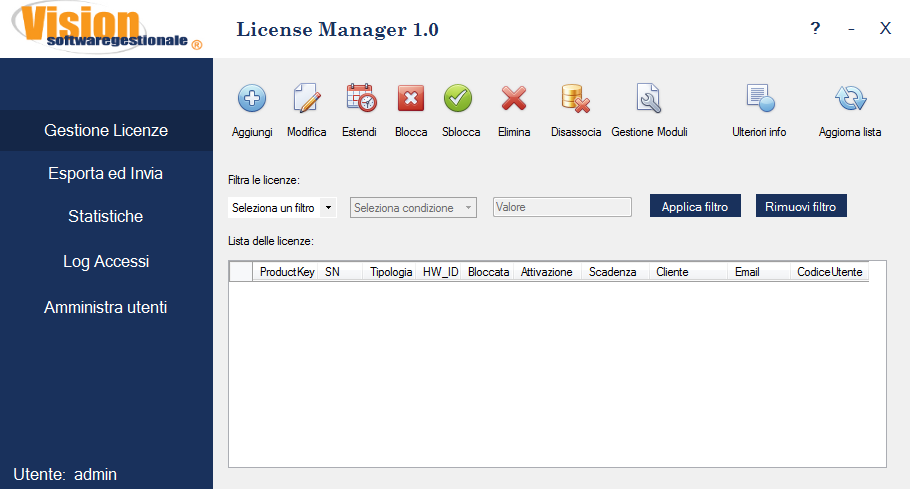
\includegraphics[width=1\columnwidth]{LicenseManager/primaSchermata} 
    \caption{License Manager 1.0 - Prima schermata all'avvio}
    \label{primscher}
\end{figure}

È presente un menu laterale, sulla sinistra, che permette la navigazione tra le diverse sezioni del programma:

\begin{itemize}
\item \textbf{Gestione Licenze:} Sono presenti tutte le funzionalità che permettono di gestire le licenze, dalla creazione all’eliminazione;
\item \textbf{Esporta ed Invia:} Sono presenti funzionalità che permettono di creare un file riepilogativo della licenza o esportare in un file Excel il riepilogo di alcuni dati;
\item \textbf{Statistiche:} Sono presenti alcune statistiche delle licenze visibili all’utente. Un \textit{Admin} può visualizzare le statistiche di tutte le licenze o di quelle associate a un rivenditore, mentre un \textit{Guest} può visualizzare le solo le statistiche delle licenze ad esso associate;
\item \textbf{Log Accessi:} Permette di visualizzare gli accessi al \textit{Software Gestionale Vision} delle proprie licenze, per monitorare eventuali anomalie;
\item \textbf{Amministra utenti:} Sezione visibile solo agli amministratori, dove è possibile gestire gli utenti del programma.

\end{itemize}

In basso a sinistra è riportato l’utente con cui si è acceduti.
\\
Tutte le sezioni saranno spiegate nel dettaglio nei prossimi paragrafi.

%**************************************************************
\newpage
\section{Gestione Licenze}
La sezione "Gestione Licenze" è la prima a mostrarsi dopo l'autenticazione. \\ In Figura \ref{gestLic} è possibile vedere una situazione esempio della sezione.

\begin{figure}[!h] 
    \centering 
    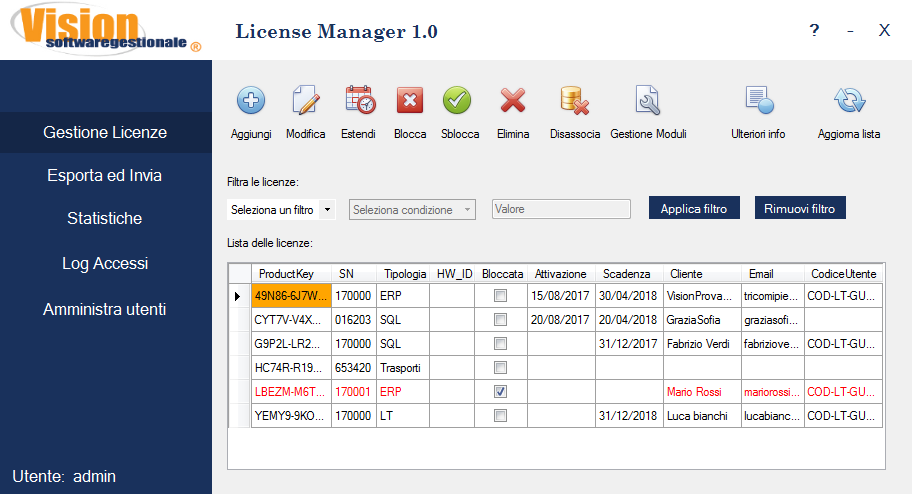
\includegraphics[width=0.9\columnwidth]{LicenseManager/gestLic} 
    \caption{License Manager 1.0 - Gestione Licenze}
\label{gestLic}
\end{figure}

Nella sezione “Gestione Licenze“ è possibile gestire tutti gli aspetti delle licenze.
Nello specifico le operazioni permesse, nell'ordine, sono:
\begin{itemize}
\item \textbf{Aggiungi:} permette di creare una nuova licenza;
\item \textbf{Modifica:} permette di modificare diversi aspetti di una licenza;
\item \textbf{Estendi:} permette di posticipare la data di scadenza;
\item \textbf{Blocca:} permette di bloccare una licenza;
\item \textbf{Sblocca:} permette di sbloccare una licenza;
\item \textbf{Elimina:} permette di eliminare una licenza;
\item \textbf{Disassocia:} permette di dissociare una licenza dalla propria componente Hardware;
\item \textbf{Gestione Moduli:} permette di gestire i moduli della licenza;
\item \textbf{Ulteriori Info:} fornisce ulteriori informazioni sulla licenza;
\item \textbf{Aggiorna lista:} permette di aggiornare la lista delle licenze;
\item \textbf{Applica filtro:} permette di filtrare le licenze in base a determinate condizioni;
\item \textbf{Rimuovi filtro:} rimuove il filtro precedentemente selezionato.
\end{itemize} 
Nella parte alta della schermata sono presenti le funzionalità, mentre nella parte bassa è mostrata la lista delle licenze visibili all’utente.
\\
Un \textit{Admin} può visualizzare tutte le licenze, ed eventualmente filtrarle per \texttt{Codice Utente} per visualizzare le licenze assegnate a un rivenditore.
\\
Un \textit{Guest} (o rivenditore), può visualizzare solo le licenze con \texttt{Codice Utente} uguale al proprio.
\\
Nei paragrafi successivi sono mostrate nel dettaglio tutte le funzionalità. 

\subsection{Aggiungi}
La funzione “Aggiungi” permette di creare una nuova licenza. Il metodo di creazione differisce per gli utenti Admin e gli utenti Guest. Cliccando sul pulsante si apre una nuova finestra, dove è possibile inserire i dati di una licenza. La finestra è riportata nella Figura \ref{crealic}.

\begin{figure}[!h] 
    \centering 
    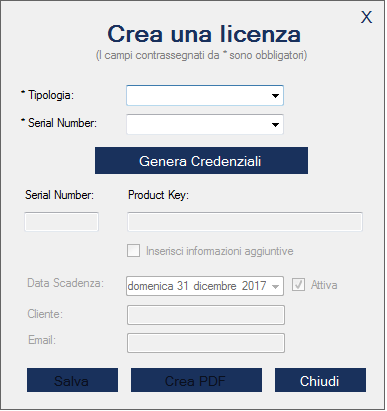
\includegraphics[width=0.55\columnwidth]{LicenseManager/creaLicenza} 
    \caption{Finestra Aggiungi - Gestione Licenze}
    \label{crealic}
\end{figure}

Per creare una licenza è necessario innanzitutto valorizzare i campi obbligatori, ovvero \texttt{Tipologia} e \texttt{Serial Number}. 
\begin{itemize}

\item \textbf{Tipologia:} Identifica quale licenza si sta creando, e i valori possibili sono SQL, LT, ERP o Trasporti. 
\item \textbf{Serial Number:} Numero di sei cifre che identifica in modo univoco, per tipologia, una licenza. Uno stesso Serial Number è permesso per diverse tipologie. La scelta del Serial Number differisce da Admin e Guest.  
\begin{itemize}

\item	\textbf{Admin:} Può scegliere tra un \texttt{Serial Number}:
\begin{itemize}
\item \textbf{Manuale:} scelto arbitrariamente;
\item \textbf{Casuale:} generato casualmente dal programma;
\item \textbf{Prime due cifre per l'anno:} le prime due cifre sono le ultime due cifre dell'anno corrente, mentre le restanti quattro identificano il punto di partenza da cui cercare un \texttt{Serial Number} libero.
\end{itemize}
\item	\textbf{Guest:} Può creare solo un \texttt{Serial Number} di tipologia “Prime due cifre per l’anno”.
\end{itemize}

\end{itemize}	

Dopo aver scelto Tipologia e Serial Number è necessario cliccare su "Genera Credenziali" per poter continuare con la creazione della licenza. Cliccando su questo pulsante è invocato un metodo del Web Service \texttt{LicenseManagerService} che produrrà un \texttt{Serial Number} compatibile con la scelta effettuata e un \texttt{Product Key} che identifica univocamente una licenza, indipendentemente dalla tipologia. Qualora il Serial Number scelto in caso di selezione "Manuale" o "Casuale" fosse già in uso, sarà comunicato che non è possibile utilizzare tali valori ed è necessario sceglierne degli altri. In caso di scelta "Prime due cifre per l’anno" il \texttt{Serial Number} prodotto sarà il primo libero disponibile a partire dal numero a quattro cifre scelto. Dopo la creazione delle credenziali il pulsante "Salva" si attiverà e sarà possibile salvare la licenza, come si evince dalla Figura \ref{salva}.

 \begin{figure}[!h] 
    \centering 
    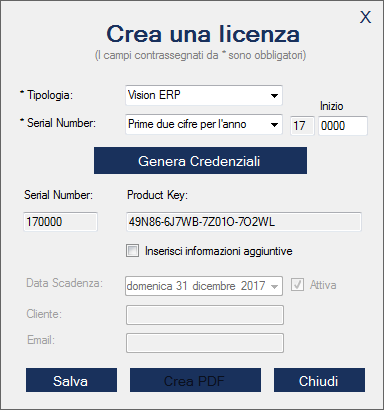
\includegraphics[width=0.55\columnwidth]{LicenseManager/salva} 
    \caption{License Manager 1.0 - Salvataggio di una licenza appena creata}
\label{salva}
\end{figure}

Prima di procedere con il salvataggio è possibile definire delle informazioni aggiuntive della licenza, come la data di scadenza, il cliente cui è destinata e l’email da associare alla licenza. La data di scadenza può essere attivata o disattivata grazie alla checkbox "Attiva" a lato del selettore della data. Nel caso di inserimento di informazioni aggiuntive è possibile anche creare direttamente il PDF contenente i dettagli della licenza da spedire al cliente. Cliccando su "Crea PDF" sarà prima chiesto di salvare la licenza.
\\Nella Figura \ref{pdf} è mostrato l'inserimento delle informazioni aggiuntive con la creazione diretta del file PDF.


\begin{figure}[!h] 
    \centering 
    \includegraphics[width=0.9\columnwidth]{LicenseManager/creaPDFInfoAggi} 
    \caption{License Manager 1.0 - Informazioni aggiuntive e creazione file PDF}
\label{pdf}
\end{figure}

Una licenza creata da un \textit{Guest} avrà come \texttt{Codice Utente} il suo codice, mentre se è creata da un \textit{Admin} esso sarà inizialmente nullo e potrà essere impostato in seguito attraverso la funzione "Modifica".
\\
Se la creazione è andata a buon fine, è mostrato un messaggio che lo conferma e la schermata di creazione viene chiusa. Nella lista delle licenze apparirà quindi la nuova licenza appena creata, come si può vedere nella Figura \ref{nuova}.

\begin{figure}[!h] 
    \centering 
    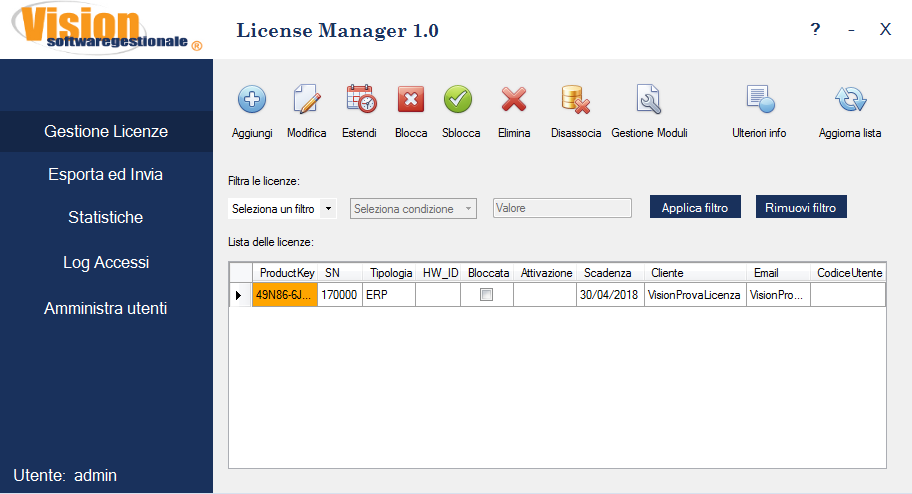
\includegraphics[width=0.9\columnwidth]{LicenseManager/nuovalicenza} 
    \caption{License Manager 1.0 - Aggiunta alla lista di una licenza appena creata}
\label{nuova}
\end{figure}

\subsection{Modifica}

La funzione "Modifica" permette di modificare i dati non immutabili di una licenza:
\begin{itemize}
\item \textbf{Data di scadenza:} data di scadenza di una licenza, può anche essere rimossa;
\item \textbf{Cliente:} nome del cliente, utilizzato per comodità per riferirsi a una licenza;
\item \textbf{Email:} indirizzo email associato alla licenza. Tramite l’indirizzo email il cliente può disattivare e riattivare la propria licenza senza che sia necessario contattare l’azienda. Per questo motivo ai \textit{Guest} non è data la possibilità di modificare l’email decisa dai clienti in fase di attivazione;
\item \textbf{Codice Utente:} codice del rifornitore cui è assegnata la licenza. Un rifornitore sarà in grado di vedere solo le licenze con il codice utente uguale a quello a lui assegnato. Per questo motivo anche il \texttt{Codice Utente} non può essere modificato dai rifornitori.
Gli \textit{Admin}, invece, possono vedere tutte le licenze e modificarne il \texttt{Codice Utente}, a meno che la licenza non sia impostata come "Licenza ad uso interno non rivendibile". Riferirsi alla sezione x.x per ulteriori informazioni.
\end{itemize} 

In Figura \ref{modifica} è mostrata la schermata di modifica.

\begin{figure}[!h] 
    \centering 
    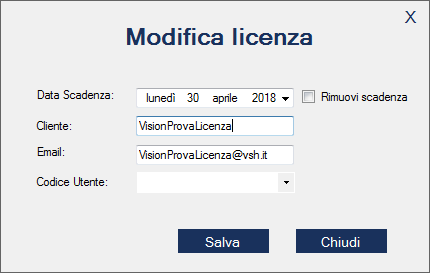
\includegraphics[width=0.6\columnwidth]{LicenseManager/modifica} 
    \caption{License Manager 1.0 - Modifica di una licenza}
\label{modifica}
\end{figure}

\subsection{Estendi}
La funzione "Estendi" permette di modificare velocemente la data di scadenza, scegliendone una nuova o indicando il numero di mesi di cui si vuole estendere la licenza.
Il Form relativo è mostrato in Figura \ref{estendi}.

\begin{figure}[!h] 
    \centering 
    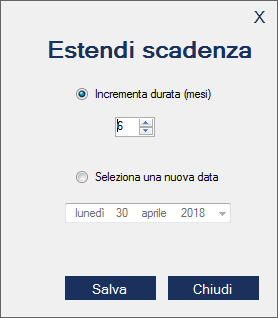
\includegraphics[width=0.45\columnwidth]{LicenseManager/Estendi} 
    \caption{License Manager 1.0 - Estensione del periodo di validità di una licenza}
\label{estendi}
\end{figure}


\subsection{Blocca}

La funzione "Blocca" permette di bloccare una licenza. All’accesso del \textit{Software Gestionale Vision} se la licenza è bloccata viene mostrato un messaggio d’errore e non è permesso l’utilizzo.
Le licenze bloccate sono mostrate in rosso nella lista delle licenze, cosi come le licenze scadute.
È possibile anche bloccare più licenze in una volta selezionandole dalla lista.
\\
Nella Figura \ref{block} si può vedere un esempio di licenza bloccata.
\begin{figure}[!h] 
    \centering 
    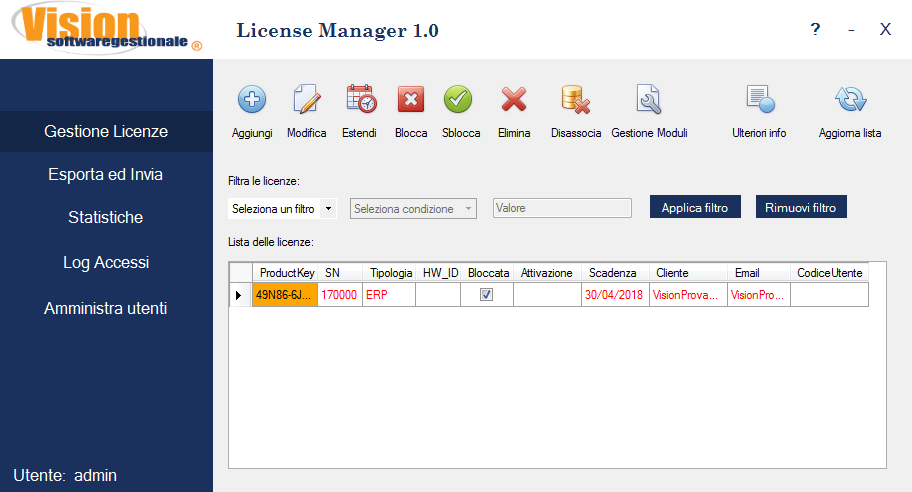
\includegraphics[width=0.9\columnwidth]{LicenseManager/bloccate} 
    \caption{License Manager 1.0 - Licenza bloccata}
\label{block}
\end{figure}

\subsection{Sblocca}
La funzione "Sblocca" permette di sbloccare una licenza bloccata in precedenza.
I rivenditori possono sbloccare solo le licenze da loro bloccate, per evitare di rimuovere i blocchi imposti dagli \textit{Admin}.\\
Come si vede nella Figura \ref{sblocca}, accedendo con un utente di tipo \textit{Guest} (in questo caso “ProvaLT”), non è possibile sbloccare una licenza bloccata da un \textit{Admin}.

\begin{figure}[!h] 
    \centering 
    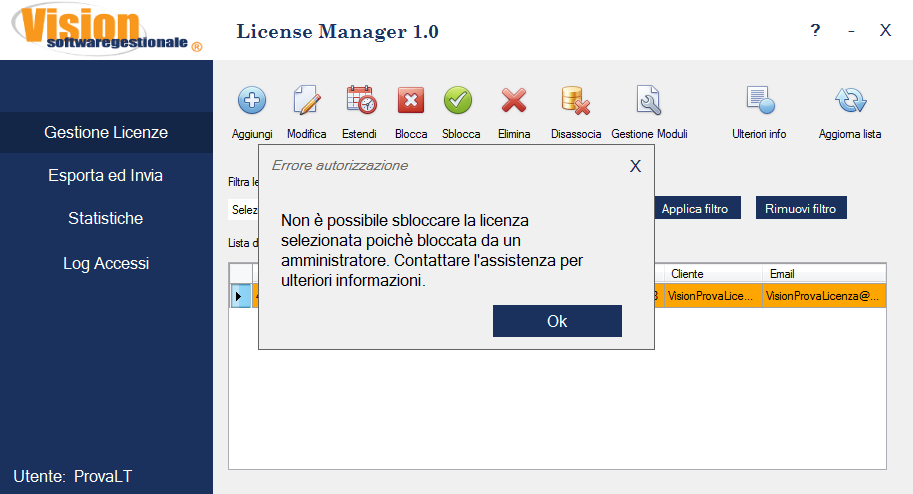
\includegraphics[width=0.9\columnwidth]{LicenseManager/sblocca} 
    \caption{License Manager 1.0 - Sblocco di una licenza}
\label{sblocca}
\end{figure}

\subsection{Elimina}
La funzione “Elimina” permette di rimuovere una licenza, tuttavia agisce in modo diverso se a richiedere l'eliminazione è un \textit{Admin} o un \textit{Guest}. Mentre per l’\textit{Admin} l’eliminazione è sempre concessa, un \textit{Guest} può eliminare la licenza solo se non è mai stata attivata o se non sono ancora stati definiti i moduli per quella licenza.\\
Nella figura \ref{elim} l’utente \textit{Guest} "ProvaLT" sta tentando l’eliminazione dopo che i moduli della licenza sono stati definiti. Il programma mostra quindi un messaggio d’errore e l’eliminazione non avviene.

\begin{figure}[!h] 
    \centering 
    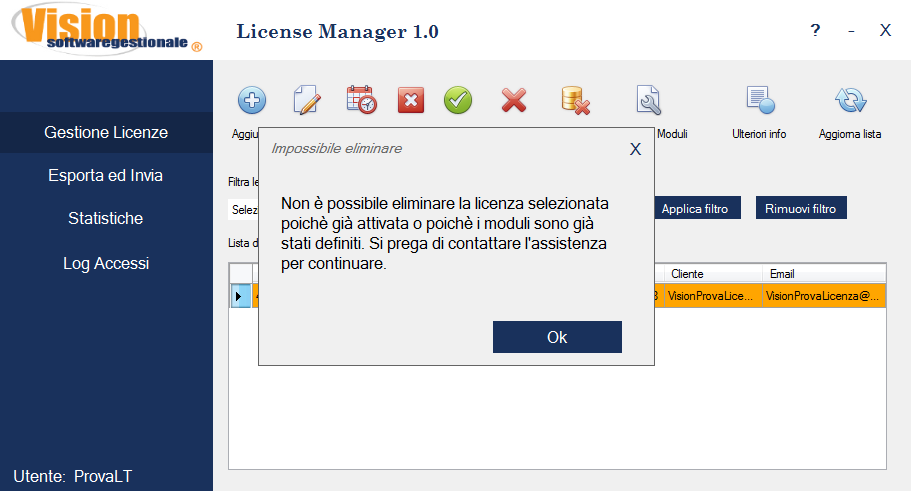
\includegraphics[width=0.9\columnwidth]{LicenseManager/elimin} 
    \caption{License Manager 1.0 - Eliminazione di una licenza}
\label{sblocca}
\end{figure}

dire che salvataggio stato, anche per le altre cose.


%**************************************************************

\section{Esporta ed Invia}

%**************************************************************
\section{Statistiche}


%**************************************************************
\section{Log Accessi}


%**************************************************************
\section{Amministra Utenti}

